%KELOMPOK 4 Blank-On1
%\begin{enumerate}
%\item Andri Fajar Sunandhar
%\item Cokro Edi Prawiro
%\item Fadila
%\item Sandro Samuel Sinaga
%\end{enumerate}


\section{Definisi Frontend}
frontend bisa disebut tampilan utama dari sebuah website pada frontend biasanya ditampilkan beberapa konten-konten yang bisa diakses oleh pengguna atau user yang menggunakan website tersebut. frontend juga berfungsi untuk user interace dari setiap web site. Biasanya frontend hanya menampilkan fungsi fungsi dari kontent sebuah web site seperti fungsi sebuah tombol untuk mengirim berkas atau untuk menampilkan konten konten yang lainnya dalam website tersebut.

Front-end adalah  segala sesuatu yang menghubungkan antara user dengan sistem back-end. Biasanya merupakan sebuah user interface 
dimana user akan berinteraksi dengan sistem. Pekerjaan yang sering muncul sebagai seorang front-end developer adalah desainer user interface
dan desainer user experience. Seorang front-end developer tidak akan membuat program atau aplikasinya yang berjalan di logic bisnis 
tapi fokusnya akan lebih banyak ke antarmuka, desain grafis (user interface designer) dan bagaimana membuat desain yang nyaman
digunakan oleh user (user experience designer). Bahasa pemrograman yang biasanya digunakan dalam pengembangan front-end adalah HTML.
\subsection{Fungsi Front-end}
Fungsi ini berhubungan langsung dengan pengguna dan berperan penting dalam keseluruhan proses bisnis dalam hal menghubungkan 
back-end dengan pengguna. layanan depan (front-end) bertugas mempresentasikan apa yang sudah dikerjakan oleh back-end
dan menjadi sarana bagi pengguna untuk mendapatkan segala sesuatu yang disediakan dibagian fungsi back-end. Peningkatan fungsi layanan depan yang baik akan mampu meningkatkan kepuasan pengguna.\cite{razaq2014sistem}
\subsection{Programming language on Front-end: Javascript }
Frontend programming language there are various. Such as HTML, CSS, and Javascript. One of them is Javascript. Javascript is language in the form of a script that in its function can run on an HTML document, where throughout history this language is the first scripting language in development / for the web. Javascript is a programming language that provides additional capabilities against the HTML language by allowing the execution of commands on the user side, which is interpreted on the browser side rather than on the server side of the web.\cite{alamsyah2003pengantar}
\subsection{Programming language on Front-end: CSS }
Frontend programming languages other than HTML, Javascript, and others, there is called CSS. CSS stands for Cascading Style Sheet. Cascading Style Sheet itself is a technology used to beautify 
the look of the website pages (sites) that you want. Using the CSS method you can easily change the overall color and appearance of the site you create, as well as to format or change the order of your site quickly.\cite{poetra2003tutorial}
\subsection{Front-end di Android}
Di Android terdapat 2 bagian, yaitu aplikasi front-end dan back-end. Front-end adalah aplikasi yang sudah terinstal dalam perangkat mobile yang digunakan.
Back-end adalah aplikasi pendukung yang berfungsi sebagai penyuplai atau sumber data pada aplikasi front-end. Front-end merupakan suatu penghubung
antara user dengan basisdata yang digunakan untuk melakukan pemrosesan data yang disimpan. Front-end dapat diciptakan menggunakan 
beberapa bahasa program seperti Visual Basic, Visual C++, Visual Foxpro, Java, dan sebagainya. Sedangkan back-end merupakan basisdata itu sendiri.
 Secara garis besar aplikasi Front-end dibagi menjadi 2 kategori, yaitu :
1. Decision Support Front-end yaitu aplikasi yang hanya menampilkan  dan mencetak informasi yang diambil dari basisdata baik melalui predefined atau user defined Query.
2. Transaction Processing front-end yaitu aplikasi yang mencakup kemampuan untuk mengedit, menambah, dan menghapus record dari basisdata.\cite{nuari2014perancangan}
\section{Konsep Membangun Aplikasi Frontend Berbasis Web APPML(Application Modeling Language) }
Diperlukan sebuah metode penghubung antara sistem dengan dukungan JSON, XML. Dengan teknik APPML (Application Modeling Language) yang diterapkan pada sebuah aplikasi front-end berbasis HTML 5 tanpa melakukan koneksi database secara langsung, tetapi cukup memanggil service berbasis JSON maka akan diperoleh data atau informasi yang dibutuhkan tanpa harus mengunjungi sistem informasi yang ada secara langsung.\cite{triyono2017konsep}

\section{definisi web serfice }
Webservice terdiri dari 2 kata yaitu Web yang berati websit atau online 
sedangangkan service berarti layanan atau melayani aplikasi berbasis web 
Website adalah suatu sistem perangkat lunak yang dirancang untuk mendukung interaksi antara sisitem pada suatu jaringan.
web service digunakan sebagai suatu fasilitas yang di sediakan oleh suatu website untuk menyediakan layanan berupa informasi kepada 
sistem lain, sehingga sisitem lain dapat berinteraksi dengan sistem tersebut melalui service yang telah disediakan oleh sistem web service.
Webservice menyimpan data informasi dalam bentuk XML, sehingga data tersebut dapat diakses oleh sitemlain miskipun berbentuk platfrom. 
\subsection{keterkaitan web service dan front end }
sebagian besar orang sering berpikir bahwa suatu website dimiliki oleh suatu pihak 
itu merupakan suatu yang disebut dengan website. banyak yang berpikir bahwa aplikasi yamg berbasiskan 
web merupakan suatu aplikasi yang menitik beratkan tampilan front endnya pada suatu web browser 
padahal nyatanya aplikasi berbasis web tidak sepenuhnya menggunakan web browser sebagai tampilan 
frontendnya. menurut Gani pengertian website di sini atalah suatu jaringan yang luas atau keterhubungan 
antara beberapa aplikasi dan atau komponen suatu aplikasi menjadi suatu aplikasi yang baru.
\subsection{Arsitektur Web Service}
\begin{figure}[ht]
\centerline{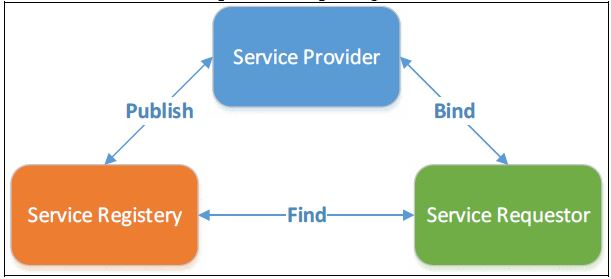
\includegraphics[width=1\textwidth]{figures/1arsitektur.JPG}}
\caption{Arsitektur web service.}
\end{figure}
terdapat tiga komponen utama dari web service, komponen komponen tersebut antara lain :
service Provider, Service Requestor, Service Registry 
service Provider adalah penyedia web service yang berfungsi menyediakan kumpulan webService yang dapat diakses oleh USER atau pengguna.
Service Requestor Adalah aplikasi yang bertindak sebagai pengguan yang melakukan permintaan layanan berupa WebService kepada Service Provider.
Service Registry Adalahtempat dimana service provider mempublikasikan layanannya. pada arsitektur Webservice, service registry bersipat opsional.\cite{kurniawan2015implementasi}


ini merupakan contoh tabel \ref{table:contoh} ukuran kecil.
\begin{table}[h]
\caption{Bahasa pemerograman yang sering digunakan di Frontend}
\centering
\begin{tabular}{ccccc}
\hline
one&two&three&four&five\\
\hline
Java&Phyton&PHP&Javascript&C++\\
\hline
\end{tabular}
\label{table:contoh}
\end{table}



